\clearpage
\SourceLeaf{233}%
\begin{center}\Large\textsc{Zur Astralgeometrie.}\end{center}
\bigskip
\begin{center}[I.]\end{center}
Die Hauptmomente des Beweises, dass die Summe der Dreieckswinkel von $180^{0}$ um eine dem Flächeninhalt proportionale Differenz verschieden ist, beruhen auf Folgendem:
\begin{center}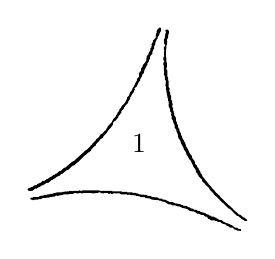
\begin{tikzpicture}[x=0.00657895cm,y=-0.00657895cm]
\fill[even odd rule] (30,341) -- (31,343) -- (34,343) -- (35,344) -- (37,344) -- (38,343) -- (45,343) -- (46,342) -- (50,342) -- (54,340) -- (67,339) -- (68,338) -- (77,337) -- (80,335) -- (84,336) -- (85,335) -- (89,335) -- (90,334) -- (93,334) -- (94,333) -- (104,333) -- (105,332) -- (112,332) -- (116,330) -- (118,330) -- (119,331) -- (124,331) -- (125,330) -- (128,330) -- (129,331) -- (131,331) -- (132,330) -- (148,330) -- (149,331) -- (155,331) -- (156,330) -- (161,330) -- (162,329) -- (165,329) -- (169,331) -- (172,331) -- (173,330) -- (179,330) -- (182,332) -- (184,331) -- (186,331) -- (187,332) -- (189,332) -- (190,331) -- (203,331) -- (206,333) -- (217,333) -- (218,334) -- (222,333) -- (223,334) -- (234,335) -- (235,336) -- (238,336) -- (239,337) -- (242,337) -- (243,338) -- (251,338) -- (253,340) -- (262,341) -- (265,343) -- (278,344) -- (279,345) -- (282,345) -- (286,347) -- (289,347) -- (297,352) -- (301,352) -- (304,354) -- (310,354) -- (314,356) -- (318,356) -- (324,359) -- (333,361) -- (338,365) -- (346,366) -- (350,368) -- (352,370) -- (355,370) -- (359,372) -- (365,373) -- (368,376) -- (371,376) -- (374,380) -- (377,381) -- (379,383) -- (386,383) -- (387,384) -- (390,384) -- (392,386) -- (397,386) -- (400,389) -- (407,391) -- (409,393) -- (412,394) -- (416,397) -- (421,397) -- (425,401) -- (427,401) -- (430,403) -- (434,403) -- (435,404) -- (437,403) -- (437,401) -- (436,400) -- (433,400) -- (428,397) -- (425,397) -- (420,393) -- (412,389) -- (410,389) -- (402,385) -- (400,383) -- (395,382) -- (384,376) -- (380,376) -- (378,374) -- (376,374) -- (374,372) -- (370,371) -- (368,369) -- (359,367) -- (357,365) -- (353,365) -- (351,363) -- (347,363) -- (345,361) -- (340,360) -- (338,358) -- (336,358) -- (331,355) -- (326,355) -- (324,353) -- (321,353) -- (320,352) -- (309,350) -- (305,348) -- (300,348) -- (290,343) -- (286,343) -- (284,341) -- (279,341) -- (276,339) -- (265,338) -- (262,336) -- (257,336) -- (254,334) -- (241,333) -- (237,331) -- (234,331) -- (233,330) -- (228,330) -- (227,329) -- (217,329) -- (216,328) -- (207,328) -- (206,327) -- (188,327) -- (187,326) -- (164,326) -- (163,325) -- (131,325) -- (130,326) -- (127,326) -- (125,325) -- (124,326) -- (112,326) -- (111,327) -- (106,326) -- (105,327) -- (101,327) -- (100,328) -- (97,327) -- (96,328) -- (92,328) -- (91,329) -- (81,329) -- (80,330) -- (74,331) -- (73,332) -- (68,332) -- (67,333) -- (63,333) -- (62,334) -- (57,334) -- (56,335) -- (49,336) -- (46,338) -- (36,338) -- (35,339) -- (32,339) -- cycle
(292,15) -- (291,16) -- (292,21) -- (291,22) -- (290,31) -- (288,34) -- (288,37) -- (289,38) -- (288,41) -- (291,45) -- (291,46) -- (288,49) -- (288,54) -- (289,55) -- (289,57) -- (288,58) -- (289,60) -- (288,62) -- (289,66) -- (287,68) -- (287,73) -- (289,76) -- (289,77) -- (287,79) -- (287,83) -- (288,84) -- (288,95) -- (289,96) -- (288,101) -- (290,105) -- (290,111) -- (292,114) -- (291,123) -- (292,124) -- (293,136) -- (294,137) -- (294,141) -- (295,142) -- (295,146) -- (296,147) -- (296,152) -- (297,153) -- (297,156) -- (298,157) -- (297,159) -- (297,162) -- (300,168) -- (300,172) -- (303,176) -- (302,178) -- (302,180) -- (303,181) -- (303,187) -- (306,191) -- (306,193) -- (309,200) -- (309,204) -- (312,208) -- (312,210) -- (315,217) -- (316,224) -- (320,229) -- (321,234) -- (326,243) -- (326,245) -- (331,252) -- (332,257) -- (334,259) -- (337,265) -- (340,268) -- (346,281) -- (348,283) -- (350,287) -- (350,290) -- (353,293) -- (353,295) -- (355,297) -- (355,298) -- (362,305) -- (362,307) -- (368,313) -- (368,314) -- (375,320) -- (377,324) -- (384,331) -- (384,332) -- (413,360) -- (416,361) -- (423,368) -- (424,370) -- (425,370) -- (429,374) -- (432,375) -- (439,381) -- (442,382) -- (444,384) -- (448,384) -- (449,383) -- (448,381) -- (447,381) -- (444,378) -- (441,377) -- (435,372) -- (433,372) -- (427,366) -- (426,366) -- (421,361) -- (421,360) -- (420,360) -- (414,354) -- (413,354) -- (403,344) -- (403,343) -- (401,342) -- (396,337) -- (396,336) -- (387,328) -- (387,327) -- (380,320) -- (380,319) -- (374,313) -- (374,312) -- (366,303) -- (366,302) -- (363,299) -- (361,294) -- (359,292) -- (358,288) -- (356,286) -- (355,283) -- (352,280) -- (352,278) -- (348,274) -- (348,271) -- (346,267) -- (342,262) -- (342,259) -- (338,254) -- (333,243) -- (331,241) -- (329,233) -- (327,231) -- (327,229) -- (325,227) -- (323,223) -- (323,221) -- (321,218) -- (321,216) -- (318,210) -- (318,207) -- (315,203) -- (315,199) -- (313,196) -- (313,194) -- (311,190) -- (311,185) -- (308,180) -- (308,176) -- (307,175) -- (307,172) -- (306,171) -- (306,167) -- (304,164) -- (305,158) -- (304,157) -- (304,153) -- (302,150) -- (302,143) -- (300,140) -- (300,136) -- (298,133) -- (299,131) -- (299,128) -- (297,126) -- (297,114) -- (296,113) -- (296,107) -- (295,106) -- (295,94) -- (293,91) -- (293,88) -- (294,87) -- (294,79) -- (293,78) -- (293,69) -- (292,68) -- (292,52) -- (293,51) -- (293,45) -- (294,44) -- (294,40) -- (295,39) -- (294,37) -- (294,34) -- (296,30) -- (296,25) -- (297,24) -- (298,19) -- (296,15) -- cycle
(281,11) -- (279,11) -- (274,17) -- (274,22) -- (273,23) -- (272,31) -- (267,36) -- (267,39) -- (264,43) -- (265,46) -- (264,47) -- (264,49) -- (262,51) -- (262,55) -- (259,59) -- (258,63) -- (255,66) -- (254,74) -- (252,78) -- (247,84) -- (247,86) -- (244,90) -- (244,94) -- (240,99) -- (240,106) -- (237,109) -- (236,111) -- (236,114) -- (234,116) -- (232,121) -- (230,123) -- (230,125) -- (227,129) -- (227,131) -- (222,137) -- (222,139) -- (220,143) -- (217,146) -- (217,148) -- (213,156) -- (207,162) -- (205,166) -- (202,169) -- (202,171) -- (198,176) -- (198,178) -- (196,180) -- (195,183) -- (190,188) -- (187,194) -- (180,201) -- (179,204) -- (177,206) -- (177,208) -- (175,210) -- (174,210) -- (170,215) -- (166,217) -- (163,222) -- (157,227) -- (157,228) -- (150,235) -- (150,236) -- (148,238) -- (147,238) -- (146,240) -- (139,247) -- (138,247) -- (115,268) -- (111,270) -- (98,281) -- (95,282) -- (90,287) -- (85,289) -- (81,293) -- (79,293) -- (77,295) -- (74,296) -- (72,298) -- (66,301) -- (64,303) -- (61,304) -- (59,306) -- (57,307) -- (54,307) -- (51,310) -- (44,313) -- (42,315) -- (37,316) -- (35,318) -- (27,321) -- (25,323) -- (25,324) -- (27,326) -- (34,326) -- (39,322) -- (42,322) -- (46,319) -- (49,318) -- (51,316) -- (55,315) -- (61,311) -- (66,310) -- (71,305) -- (73,305) -- (75,303) -- (78,302) -- (81,299) -- (86,297) -- (89,294) -- (92,293) -- (99,287) -- (104,285) -- (111,278) -- (116,276) -- (121,271) -- (122,271) -- (136,257) -- (137,257) -- (142,252) -- (143,252) -- (148,247) -- (148,246) -- (154,240) -- (156,239) -- (157,236) -- (164,229) -- (164,228) -- (166,226) -- (170,224) -- (172,220) -- (177,215) -- (180,210) -- (188,201) -- (190,197) -- (190,194) -- (193,191) -- (194,191) -- (200,184) -- (200,182) -- (206,175) -- (206,172) -- (211,167) -- (211,165) -- (213,163) -- (213,162) -- (219,156) -- (219,154) -- (223,148) -- (223,145) -- (225,143) -- (226,140) -- (230,135) -- (230,133) -- (232,131) -- (231,128) -- (235,125) -- (240,115) -- (242,113) -- (242,111) -- (246,104) -- (246,102) -- (249,99) -- (251,91) -- (253,89) -- (253,87) -- (256,83) -- (256,80) -- (259,76) -- (259,74) -- (261,71) -- (261,68) -- (263,64) -- (266,61) -- (266,57) -- (267,56) -- (267,54) -- (269,52) -- (269,47) -- (271,44) -- (272,38) -- (274,34) -- (276,32) -- (276,29) -- (279,25) -- (280,21) -- (282,18) -- (282,12) -- cycle;
\node[inner sep=0pt] at (240,235) {$1$};
\end{tikzpicture}
\hspace{1em}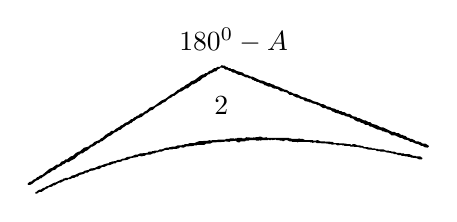
\begin{tikzpicture}[x=0.00739191cm,y=-0.00739191cm]
\fill[even odd rule] (691,255) -- (687,252) -- (680,252) -- (679,251) -- (675,251) -- (668,248) -- (660,248) -- (659,247) -- (654,247) -- (653,246) -- (647,246) -- (643,244) -- (638,244) -- (637,243) -- (634,243) -- (633,242) -- (628,242) -- (624,240) -- (615,240) -- (614,239) -- (610,239) -- (609,238) -- (604,238) -- (603,237) -- (598,237) -- (597,236) -- (591,236) -- (588,234) -- (585,234) -- (584,233) -- (579,233) -- (575,231) -- (571,231) -- (570,232) -- (568,232) -- (567,231) -- (561,231) -- (560,230) -- (539,229) -- (536,227) -- (515,226) -- (511,224) -- (509,224) -- (508,225) -- (503,225) -- (502,224) -- (489,224) -- (485,222) -- (480,222) -- (479,221) -- (477,222) -- (466,222) -- (465,221) -- (462,221) -- (461,220) -- (424,220) -- (423,219) -- (417,220) -- (413,218) -- (410,218) -- (409,219) -- (404,219) -- (403,220) -- (401,219) -- (399,220) -- (388,219) -- (385,221) -- (381,221) -- (380,220) -- (373,220) -- (372,221) -- (369,221) -- (368,222) -- (366,221) -- (360,221) -- (359,222) -- (353,222) -- (352,223) -- (339,223) -- (338,224) -- (329,224) -- (328,225) -- (324,224) -- (323,225) -- (306,226) -- (299,229) -- (291,229) -- (287,231) -- (282,231) -- (281,232) -- (278,232) -- (277,233) -- (270,233) -- (266,235) -- (260,235) -- (259,236) -- (256,236) -- (255,237) -- (250,237) -- (243,240) -- (239,240) -- (236,242) -- (230,242) -- (229,243) -- (226,243) -- (225,244) -- (220,244) -- (218,246) -- (205,247) -- (201,249) -- (197,249) -- (191,252) -- (183,253) -- (178,256) -- (175,256) -- (171,258) -- (167,258) -- (163,260) -- (156,261) -- (155,262) -- (153,262) -- (151,264) -- (148,264) -- (147,265) -- (145,265) -- (138,268) -- (135,268) -- (127,272) -- (119,273) -- (117,275) -- (109,277) -- (107,279) -- (101,280) -- (93,284) -- (88,285) -- (86,287) -- (82,289) -- (77,289) -- (76,290) -- (74,290) -- (72,292) -- (70,292) -- (60,297) -- (58,297) -- (47,303) -- (45,303) -- (41,306) -- (39,306) -- (35,309) -- (33,309) -- (29,311) -- (27,313) -- (26,313) -- (25,315) -- (26,316) -- (28,316) -- (32,313) -- (36,313) -- (43,308) -- (46,307) -- (48,305) -- (54,304) -- (56,302) -- (58,302) -- (66,297) -- (69,297) -- (76,293) -- (80,293) -- (82,291) -- (85,291) -- (89,289) -- (92,289) -- (95,287) -- (98,287) -- (101,284) -- (109,282) -- (111,280) -- (115,280) -- (119,277) -- (126,276) -- (130,274) -- (135,274) -- (140,270) -- (144,270) -- (150,267) -- (153,267) -- (160,264) -- (163,264) -- (165,262) -- (173,261) -- (175,259) -- (183,258) -- (189,255) -- (201,253) -- (203,251) -- (209,252) -- (210,251) -- (213,251) -- (216,249) -- (223,249) -- (227,247) -- (230,247) -- (233,245) -- (236,245) -- (237,244) -- (242,244) -- (248,241) -- (254,241) -- (255,240) -- (261,240) -- (262,239) -- (269,239) -- (270,238) -- (272,238) -- (274,236) -- (280,237) -- (284,235) -- (297,234) -- (298,233) -- (303,233) -- (304,232) -- (316,232) -- (319,230) -- (326,230) -- (330,228) -- (350,227) -- (351,226) -- (359,227) -- (360,226) -- (369,225) -- (374,228) -- (376,228) -- (378,226) -- (386,226) -- (387,225) -- (392,225) -- (393,224) -- (404,224) -- (405,225) -- (409,225) -- (411,224) -- (413,225) -- (414,224) -- (425,224) -- (426,223) -- (428,224) -- (430,224) -- (431,223) -- (433,224) -- (439,223) -- (440,224) -- (445,224) -- (446,225) -- (450,225) -- (451,226) -- (455,224) -- (458,224) -- (462,226) -- (466,226) -- (467,227) -- (475,227) -- (476,228) -- (478,227) -- (497,227) -- (498,228) -- (501,228) -- (502,229) -- (504,228) -- (508,228) -- (509,229) -- (529,230) -- (530,231) -- (534,231) -- (535,232) -- (541,231) -- (545,233) -- (552,232) -- (553,233) -- (556,233) -- (557,234) -- (566,234) -- (567,235) -- (582,236) -- (583,237) -- (588,237) -- (589,238) -- (595,239) -- (596,240) -- (610,241) -- (613,243) -- (618,243) -- (619,244) -- (627,244) -- (628,245) -- (637,246) -- (638,247) -- (641,247) -- (642,248) -- (646,248) -- (650,250) -- (654,250) -- (655,251) -- (660,251) -- (661,252) -- (665,252) -- (666,253) -- (670,253) -- (671,254) -- (681,255) -- (685,257) -- (690,257) -- cycle
(702,234) -- (696,230) -- (691,230) -- (687,227) -- (685,227) -- (684,226) -- (679,226) -- (677,224) -- (673,222) -- (670,222) -- (667,220) -- (665,220) -- (662,217) -- (658,216) -- (657,215) -- (654,215) -- (650,212) -- (646,212) -- (643,210) -- (639,210) -- (623,202) -- (619,202) -- (612,198) -- (604,196) -- (601,193) -- (598,193) -- (593,190) -- (590,190) -- (582,186) -- (579,186) -- (577,184) -- (571,183) -- (566,179) -- (561,179) -- (557,176) -- (554,176) -- (551,174) -- (548,174) -- (546,172) -- (543,172) -- (540,170) -- (535,169) -- (532,167) -- (526,166) -- (524,164) -- (520,162) -- (517,162) -- (511,159) -- (503,157) -- (498,154) -- (493,153) -- (490,151) -- (484,150) -- (475,145) -- (469,144) -- (464,141) -- (462,141) -- (458,138) -- (453,137) -- (443,132) -- (438,131) -- (434,128) -- (432,128) -- (428,126) -- (425,126) -- (417,122) -- (411,121) -- (399,115) -- (396,115) -- (390,112) -- (385,111) -- (382,108) -- (371,105) -- (366,102) -- (362,102) -- (360,100) -- (357,100) -- (355,98) -- (353,98) -- (351,96) -- (348,96) -- (346,95) -- (343,98) -- (338,98) -- (336,100) -- (333,100) -- (328,104) -- (324,105) -- (320,109) -- (317,109) -- (315,111) -- (313,111) -- (309,113) -- (299,121) -- (293,123) -- (290,126) -- (284,129) -- (281,132) -- (276,134) -- (273,137) -- (271,137) -- (263,144) -- (258,146) -- (249,153) -- (242,156) -- (229,166) -- (222,168) -- (217,173) -- (213,175) -- (210,178) -- (207,178) -- (205,179) -- (202,182) -- (200,182) -- (198,184) -- (195,185) -- (192,188) -- (190,188) -- (184,193) -- (180,194) -- (175,198) -- (172,199) -- (170,201) -- (163,205) -- (160,208) -- (156,208) -- (152,212) -- (150,212) -- (148,214) -- (147,214) -- (141,220) -- (138,221) -- (135,224) -- (127,227) -- (123,231) -- (120,232) -- (117,235) -- (109,237) -- (101,244) -- (99,244) -- (95,246) -- (90,251) -- (86,252) -- (80,257) -- (77,257) -- (74,260) -- (70,261) -- (67,265) -- (65,266) -- (62,266) -- (54,272) -- (50,273) -- (37,284) -- (33,285) -- (31,287) -- (28,288) -- (25,291) -- (22,292) -- (19,295) -- (15,296) -- (12,299) -- (12,300) -- (13,301) -- (16,301) -- (20,299) -- (26,294) -- (31,292) -- (33,290) -- (35,290) -- (38,287) -- (39,287) -- (47,281) -- (50,280) -- (55,276) -- (59,275) -- (63,271) -- (70,268) -- (72,266) -- (75,265) -- (78,262) -- (83,262) -- (85,260) -- (93,256) -- (100,249) -- (101,249) -- (103,247) -- (106,247) -- (111,243) -- (114,242) -- (122,235) -- (124,235) -- (129,232) -- (132,229) -- (135,229) -- (138,226) -- (140,226) -- (150,218) -- (155,216) -- (161,211) -- (166,209) -- (168,207) -- (172,206) -- (176,202) -- (177,202) -- (182,198) -- (186,197) -- (188,195) -- (190,195) -- (194,191) -- (195,191) -- (200,187) -- (208,184) -- (215,178) -- (217,178) -- (223,173) -- (227,172) -- (232,167) -- (242,162) -- (244,160) -- (249,158) -- (254,153) -- (260,150) -- (262,148) -- (264,148) -- (273,141) -- (277,140) -- (284,135) -- (287,135) -- (295,128) -- (297,128) -- (303,125) -- (305,123) -- (308,122) -- (313,117) -- (318,115) -- (322,111) -- (324,111) -- (326,109) -- (328,109) -- (333,106) -- (336,106) -- (339,102) -- (342,101) -- (344,99) -- (349,100) -- (352,103) -- (356,103) -- (359,105) -- (361,105) -- (365,108) -- (368,108) -- (375,112) -- (379,112) -- (387,116) -- (390,116) -- (393,118) -- (396,118) -- (399,121) -- (401,121) -- (402,122) -- (404,122) -- (406,124) -- (409,124) -- (412,126) -- (417,127) -- (420,130) -- (422,130) -- (426,132) -- (430,132) -- (434,135) -- (442,136) -- (447,140) -- (452,140) -- (453,141) -- (458,142) -- (462,146) -- (467,146) -- (469,148) -- (475,151) -- (478,151) -- (481,153) -- (486,154) -- (489,157) -- (495,158) -- (496,159) -- (499,159) -- (502,161) -- (508,162) -- (510,164) -- (513,164) -- (520,169) -- (525,169) -- (527,171) -- (533,172) -- (536,175) -- (538,175) -- (541,177) -- (543,177) -- (544,178) -- (546,178) -- (553,181) -- (556,181) -- (559,183) -- (565,184) -- (567,186) -- (572,187) -- (575,190) -- (579,192) -- (583,192) -- (585,194) -- (589,195) -- (593,198) -- (598,198) -- (601,201) -- (604,201) -- (614,206) -- (617,206) -- (618,207) -- (620,207) -- (622,209) -- (625,209) -- (626,210) -- (632,211) -- (638,216) -- (644,216) -- (652,220) -- (655,220) -- (660,223) -- (666,224) -- (670,227) -- (673,227) -- (679,230) -- (684,231) -- (689,234) -- (692,234) -- (694,236) -- (700,237) -- (702,235) -- cycle;
\node[inner sep=0pt] at (366,52) {$180^{0}-A$};
\node[inner sep=0pt] at (345,164) {$2$};
\end{tikzpicture}
\end{center}
Inhalt des unendlichen Dreiecks $1=T$.

Inhalt des unendlichen Dreiecks $2=\varphi A$.

Dann ist
\[
\begin{aligned}
1.\quad &\varphi A+\varphi(180^{0}-A)=T,\\
2.\quad &\varphi B+\varphi C+\varphi(180^{0}-B-C)=T,
\end{aligned}
\]
beides durch Construction.

Also wenn man $A=B+C$ setzt:
\[
3.\quad\varphi B+\varphi C=\varphi(B+C),
\]
mithin $\varphi t=at$, wo $a$ ein constanter Factor und
\[
a.180^{0}=T.
\]
\Needspace{25\baselineskip}
\begin{center}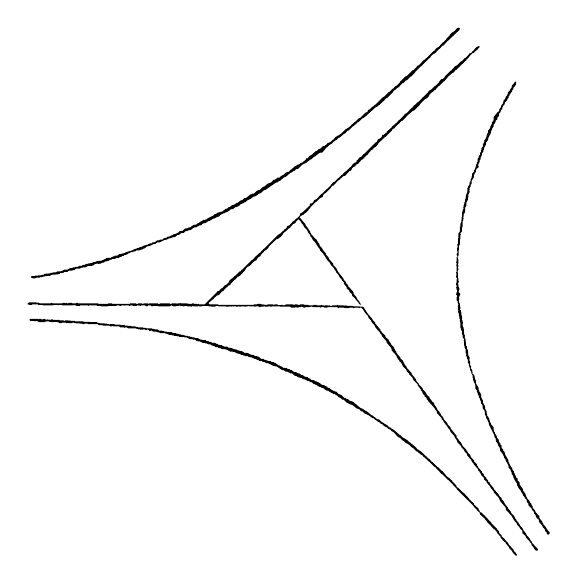
\begin{tikzpicture}[x=0.00597015cm,y=-0.00597015cm]
\fill[even odd rule] (16,636) -- (16,637) -- (18,639) -- (26,639) -- (27,640) -- (32,639) -- (36,642) -- (48,642) -- (51,640) -- (57,640) -- (58,641) -- (62,641) -- (63,642) -- (74,641) -- (81,644) -- (84,644) -- (85,643) -- (93,643) -- (94,644) -- (106,644) -- (107,643) -- (111,643) -- (112,644) -- (128,645) -- (129,646) -- (132,646) -- (133,645) -- (140,645) -- (141,646) -- (161,646) -- (163,648) -- (171,648) -- (172,649) -- (185,649) -- (188,651) -- (190,651) -- (191,650) -- (193,650) -- (194,651) -- (207,651) -- (209,653) -- (217,653) -- (218,654) -- (220,653) -- (223,653) -- (226,655) -- (243,655) -- (244,656) -- (246,656) -- (247,657) -- (251,657) -- (252,658) -- (257,658) -- (258,657) -- (261,657) -- (264,659) -- (266,658) -- (269,658) -- (272,661) -- (274,660) -- (277,660) -- (279,662) -- (286,662) -- (287,663) -- (293,664) -- (294,665) -- (304,665) -- (305,666) -- (307,666) -- (314,669) -- (319,669) -- (320,670) -- (323,670) -- (324,671) -- (330,671) -- (331,672) -- (334,672) -- (335,673) -- (340,673) -- (341,674) -- (343,673) -- (345,674) -- (350,674) -- (354,676) -- (356,678) -- (363,678) -- (364,679) -- (368,679) -- (372,682) -- (379,683) -- (385,686) -- (389,686) -- (390,687) -- (393,687) -- (397,689) -- (401,689) -- (403,691) -- (410,693) -- (412,695) -- (416,695) -- (419,697) -- (422,697) -- (426,699) -- (431,699) -- (432,700) -- (435,700) -- (445,705) -- (447,704) -- (449,705) -- (452,705) -- (457,708) -- (465,710) -- (467,712) -- (470,711) -- (472,713) -- (474,713) -- (475,714) -- (480,714) -- (483,716) -- (489,717) -- (495,720) -- (498,720) -- (500,722) -- (502,722) -- (507,725) -- (510,724) -- (512,726) -- (517,727) -- (520,729) -- (523,729) -- (535,735) -- (537,735) -- (538,736) -- (542,736) -- (554,744) -- (557,744) -- (561,747) -- (565,747) -- (567,749) -- (569,749) -- (571,751) -- (575,751) -- (581,756) -- (583,756) -- (588,759) -- (596,761) -- (598,763) -- (603,764) -- (608,767) -- (611,767) -- (613,769) -- (617,770) -- (621,774) -- (624,774) -- (626,776) -- (628,776) -- (630,778) -- (634,780) -- (636,780) -- (638,782) -- (641,782) -- (647,787) -- (652,788) -- (656,791) -- (662,794) -- (666,795) -- (668,797) -- (671,798) -- (675,802) -- (678,803) -- (682,807) -- (685,807) -- (691,813) -- (699,817) -- (703,818) -- (713,826) -- (715,826) -- (719,828) -- (722,832) -- (725,832) -- (729,836) -- (738,840) -- (746,846) -- (748,846) -- (752,850) -- (753,850) -- (758,854) -- (760,854) -- (764,858) -- (768,860) -- (771,863) -- (777,866) -- (780,869) -- (783,870) -- (787,874) -- (791,876) -- (801,887) -- (803,887) -- (805,889) -- (806,889) -- (809,893) -- (813,895) -- (818,900) -- (820,900) -- (822,902) -- (823,902) -- (829,908) -- (833,910) -- (840,917) -- (841,917) -- (848,923) -- (852,925) -- (855,929) -- (856,929) -- (861,934) -- (862,934) -- (865,938) -- (866,938) -- (878,950) -- (879,950) -- (894,966) -- (895,966) -- (907,978) -- (908,978) -- (925,996) -- (925,997) -- (962,1034) -- (962,1035) -- (968,1041) -- (968,1042) -- (974,1047) -- (975,1051) -- (986,1061) -- (986,1062) -- (990,1066) -- (990,1067) -- (999,1076) -- (999,1077) -- (1011,1088) -- (1011,1090) -- (1019,1099) -- (1019,1101) -- (1023,1105) -- (1023,1106) -- (1030,1112) -- (1030,1113) -- (1036,1120) -- (1037,1123) -- (1043,1129) -- (1045,1133) -- (1051,1139) -- (1053,1139) -- (1054,1138) -- (1051,1133) -- (1047,1129) -- (1046,1126) -- (1036,1115) -- (1034,1111) -- (1028,1105) -- (1028,1104) -- (1021,1098) -- (1021,1096) -- (1016,1091) -- (1015,1087) -- (1011,1083) -- (1011,1082) -- (999,1070) -- (999,1069) -- (992,1062) -- (992,1061) -- (986,1055) -- (986,1054) -- (984,1053) -- (978,1047) -- (976,1047) -- (974,1045) -- (974,1043) -- (972,1041) -- (972,1039) -- (962,1030) -- (962,1028) -- (952,1019) -- (952,1018) -- (940,1005) -- (939,1005) -- (928,994) -- (927,994) -- (925,992) -- (924,989) -- (916,981) -- (916,980) -- (906,971) -- (905,971) -- (895,959) -- (894,959) -- (885,950) -- (884,950) -- (873,939) -- (872,939) -- (867,933) -- (866,933) -- (848,916) -- (847,916) -- (844,913) -- (842,913) -- (840,911) -- (840,910) -- (831,902) -- (830,902) -- (826,898) -- (825,898) -- (820,893) -- (810,887) -- (805,882) -- (804,882) -- (790,870) -- (787,869) -- (784,866) -- (782,866) -- (777,861) -- (771,858) -- (769,856) -- (766,855) -- (760,849) -- (757,849) -- (755,847) -- (754,847) -- (751,844) -- (750,844) -- (747,841) -- (744,840) -- (733,831) -- (730,830) -- (725,826) -- (721,825) -- (704,811) -- (697,809) -- (694,806) -- (690,805) -- (688,803) -- (686,803) -- (680,797) -- (674,795) -- (669,790) -- (665,789) -- (659,786) -- (657,784) -- (656,784) -- (654,782) -- (652,782) -- (647,778) -- (643,776) -- (638,775) -- (633,771) -- (627,768) -- (625,768) -- (620,765) -- (616,765) -- (613,762) -- (610,761) -- (608,759) -- (602,758) -- (598,755) -- (594,754) -- (590,751) -- (587,751) -- (583,748) -- (580,748) -- (576,746) -- (574,744) -- (572,744) -- (569,742) -- (566,742) -- (564,740) -- (556,739) -- (552,736) -- (550,736) -- (548,734) -- (546,734) -- (541,730) -- (535,727) -- (532,727) -- (529,725) -- (525,725) -- (524,724) -- (516,722) -- (514,720) -- (509,720) -- (503,715) -- (501,715) -- (500,714) -- (496,714) -- (493,712) -- (487,711) -- (479,707) -- (473,707) -- (469,704) -- (463,703) -- (462,702) -- (459,702) -- (456,700) -- (453,700) -- (446,697) -- (439,696) -- (437,694) -- (431,694) -- (425,691) -- (418,690) -- (416,688) -- (414,688) -- (410,686) -- (405,686) -- (402,684) -- (399,684) -- (396,682) -- (393,682) -- (390,680) -- (384,680) -- (383,679) -- (380,679) -- (374,676) -- (369,676) -- (366,674) -- (362,674) -- (361,673) -- (358,673) -- (357,672) -- (353,672) -- (352,671) -- (348,671) -- (347,670) -- (344,670) -- (343,669) -- (339,669) -- (338,668) -- (335,668) -- (334,667) -- (328,666) -- (327,665) -- (322,665) -- (318,663) -- (309,663) -- (308,662) -- (303,662) -- (302,661) -- (299,661) -- (298,660) -- (292,660) -- (288,657) -- (282,657) -- (281,656) -- (277,656) -- (276,655) -- (265,655) -- (264,654) -- (258,654) -- (257,653) -- (247,653) -- (246,652) -- (242,652) -- (241,651) -- (233,651) -- (232,650) -- (225,650) -- (224,649) -- (219,649) -- (218,648) -- (210,648) -- (209,647) -- (197,647) -- (196,646) -- (188,646) -- (186,647) -- (185,646) -- (182,646) -- (181,645) -- (162,644) -- (159,642) -- (145,642) -- (144,641) -- (131,641) -- (130,640) -- (113,640) -- (112,639) -- (103,639) -- (102,638) -- (100,639) -- (98,638) -- (92,638) -- (91,639) -- (89,639) -- (88,638) -- (80,638) -- (79,637) -- (76,637) -- (74,638) -- (73,637) -- (66,637) -- (65,636) -- (62,636) -- (61,637) -- (53,636) -- (51,637) -- (48,635) -- (46,635) -- (45,636) -- (41,636) -- (40,635) -- (37,635) -- (36,636) -- (34,635) -- (17,635) -- cycle
(1049,130) -- (1047,134) -- (1044,137) -- (1042,141) -- (1042,143) -- (1040,145) -- (1038,149) -- (1034,153) -- (1034,156) -- (1032,160) -- (1030,162) -- (1028,167) -- (1025,170) -- (1024,176) -- (1020,181) -- (1019,185) -- (1016,188) -- (1016,191) -- (1015,193) -- (1010,197) -- (1010,198) -- (1004,205) -- (1004,212) -- (1000,217) -- (1000,220) -- (997,225) -- (997,227) -- (995,231) -- (992,234) -- (992,239) -- (990,241) -- (988,249) -- (986,253) -- (984,255) -- (984,258) -- (981,264) -- (981,268) -- (978,272) -- (978,275) -- (977,276) -- (977,279) -- (975,282) -- (975,285) -- (972,289) -- (972,292) -- (970,294) -- (970,300) -- (968,302) -- (968,305) -- (967,306) -- (964,317) -- (962,319) -- (962,322) -- (958,326) -- (958,331) -- (957,332) -- (957,335) -- (955,338) -- (955,342) -- (953,344) -- (952,350) -- (949,354) -- (949,356) -- (948,357) -- (948,365) -- (945,372) -- (945,376) -- (944,377) -- (944,380) -- (943,381) -- (943,385) -- (942,386) -- (941,392) -- (940,393) -- (940,397) -- (939,398) -- (940,401) -- (938,403) -- (938,406) -- (937,407) -- (937,417) -- (936,418) -- (935,429) -- (933,433) -- (933,439) -- (932,440) -- (932,449) -- (929,453) -- (928,475) -- (926,477) -- (927,479) -- (927,483) -- (926,484) -- (926,491) -- (927,492) -- (927,494) -- (925,497) -- (925,499) -- (927,501) -- (927,502) -- (925,504) -- (925,513) -- (924,514) -- (925,516) -- (925,519) -- (924,520) -- (925,522) -- (925,535) -- (924,536) -- (925,542) -- (924,543) -- (924,546) -- (926,548) -- (926,550) -- (925,551) -- (925,558) -- (924,559) -- (924,563) -- (925,564) -- (925,567) -- (924,569) -- (925,570) -- (925,573) -- (926,574) -- (926,578) -- (925,579) -- (924,583) -- (926,585) -- (926,588) -- (925,589) -- (925,595) -- (927,597) -- (927,600) -- (929,604) -- (928,606) -- (928,615) -- (929,616) -- (928,620) -- (930,624) -- (930,629) -- (931,630) -- (931,634) -- (932,635) -- (932,641) -- (933,642) -- (933,653) -- (934,654) -- (934,657) -- (937,662) -- (936,666) -- (938,670) -- (938,674) -- (941,678) -- (941,680) -- (940,681) -- (941,683) -- (941,690) -- (942,691) -- (941,692) -- (942,693) -- (942,696) -- (944,699) -- (944,707) -- (946,709) -- (945,713) -- (947,716) -- (947,718) -- (949,722) -- (949,728) -- (951,730) -- (951,734) -- (954,741) -- (954,744) -- (956,747) -- (957,752) -- (959,755) -- (959,760) -- (960,761) -- (960,764) -- (965,776) -- (965,783) -- (968,787) -- (968,789) -- (969,790) -- (970,795) -- (972,798) -- (973,803) -- (975,805) -- (975,807) -- (977,811) -- (977,815) -- (980,818) -- (981,826) -- (984,829) -- (984,831) -- (985,832) -- (985,837) -- (988,843) -- (988,846) -- (991,850) -- (991,852) -- (993,855) -- (994,860) -- (1005,882) -- (1006,887) -- (1008,889) -- (1009,896) -- (1012,899) -- (1013,903) -- (1015,907) -- (1017,909) -- (1018,916) -- (1023,922) -- (1026,928) -- (1026,930) -- (1029,934) -- (1030,938) -- (1032,940) -- (1035,946) -- (1036,952) -- (1040,956) -- (1040,958) -- (1042,961) -- (1042,965) -- (1044,967) -- (1046,971) -- (1046,973) -- (1048,975) -- (1048,977) -- (1054,986) -- (1054,989) -- (1057,995) -- (1062,1001) -- (1063,1004) -- (1066,1008) -- (1066,1010) -- (1070,1014) -- (1070,1016) -- (1074,1020) -- (1075,1025) -- (1078,1028) -- (1078,1031) -- (1079,1033) -- (1085,1039) -- (1085,1041) -- (1090,1046) -- (1090,1049) -- (1093,1052) -- (1093,1054) -- (1096,1059) -- (1100,1062) -- (1100,1065) -- (1102,1069) -- (1106,1073) -- (1109,1079) -- (1113,1083) -- (1114,1087) -- (1117,1090) -- (1117,1092) -- (1119,1094) -- (1121,1094) -- (1123,1092) -- (1123,1089) -- (1119,1085) -- (1114,1077) -- (1110,1073) -- (1110,1071) -- (1108,1069) -- (1107,1066) -- (1102,1060) -- (1101,1058) -- (1101,1055) -- (1093,1046) -- (1092,1043) -- (1087,1037) -- (1087,1034) -- (1085,1032) -- (1084,1028) -- (1081,1025) -- (1080,1022) -- (1076,1018) -- (1072,1010) -- (1072,1008) -- (1066,1000) -- (1066,997) -- (1059,987) -- (1059,983) -- (1055,979) -- (1055,975) -- (1051,972) -- (1051,969) -- (1049,967) -- (1049,965) -- (1047,962) -- (1047,959) -- (1044,956) -- (1044,954) -- (1041,950) -- (1035,938) -- (1035,935) -- (1029,925) -- (1027,918) -- (1024,915) -- (1024,913) -- (1021,910) -- (1021,905) -- (1018,902) -- (1018,900) -- (1016,898) -- (1014,891) -- (1011,888) -- (1011,886) -- (1009,882) -- (1007,880) -- (1007,877) -- (1005,875) -- (1005,873) -- (1004,872) -- (1004,866) -- (998,859) -- (998,857) -- (996,854) -- (994,846) -- (990,841) -- (990,838) -- (989,837) -- (989,832) -- (986,827) -- (986,822) -- (981,813) -- (981,809) -- (977,801) -- (977,796) -- (976,795) -- (976,793) -- (973,789) -- (973,787) -- (972,786) -- (972,782) -- (966,772) -- (966,766) -- (964,763) -- (963,756) -- (962,754) -- (958,751) -- (959,749) -- (958,743) -- (955,740) -- (956,736) -- (954,734) -- (954,727) -- (952,723) -- (953,717) -- (950,713) -- (949,702) -- (947,698) -- (947,694) -- (945,691) -- (944,678) -- (942,674) -- (943,671) -- (941,667) -- (940,654) -- (938,650) -- (938,645) -- (939,643) -- (938,642) -- (938,639) -- (936,637) -- (937,632) -- (936,631) -- (936,628) -- (935,627) -- (935,621) -- (934,620) -- (934,617) -- (932,615) -- (933,613) -- (933,609) -- (932,608) -- (932,603) -- (930,599) -- (930,594) -- (931,593) -- (930,589) -- (933,582) -- (929,578) -- (930,574) -- (931,573) -- (931,570) -- (929,566) -- (929,561) -- (928,560) -- (928,558) -- (930,556) -- (930,555) -- (929,554) -- (929,549) -- (928,548) -- (928,537) -- (927,536) -- (927,533) -- (929,530) -- (929,528) -- (928,527) -- (928,524) -- (929,523) -- (929,521) -- (928,520) -- (928,518) -- (929,517) -- (929,508) -- (928,507) -- (927,503) -- (929,501) -- (930,480) -- (932,476) -- (932,466) -- (933,465) -- (933,457) -- (934,456) -- (933,452) -- (936,449) -- (936,441) -- (938,438) -- (938,427) -- (939,426) -- (939,423) -- (940,422) -- (939,418) -- (940,417) -- (940,412) -- (943,408) -- (943,398) -- (946,394) -- (946,387) -- (949,381) -- (949,377) -- (950,376) -- (950,373) -- (949,371) -- (951,369) -- (951,367) -- (953,365) -- (952,361) -- (953,360) -- (953,356) -- (955,353) -- (955,349) -- (957,347) -- (957,341) -- (962,333) -- (962,329) -- (963,328) -- (963,326) -- (966,322) -- (966,319) -- (968,315) -- (972,312) -- (971,306) -- (974,301) -- (974,297) -- (976,295) -- (976,292) -- (979,286) -- (979,282) -- (982,279) -- (982,276) -- (983,275) -- (984,270) -- (987,265) -- (988,259) -- (992,254) -- (992,251) -- (998,239) -- (998,235) -- (1000,233) -- (1001,229) -- (1004,225) -- (1004,221) -- (1006,219) -- (1008,215) -- (1008,213) -- (1012,210) -- (1012,206) -- (1015,203) -- (1015,198) -- (1018,195) -- (1020,190) -- (1022,188) -- (1024,181) -- (1027,178) -- (1028,174) -- (1033,169) -- (1033,167) -- (1036,164) -- (1036,161) -- (1038,159) -- (1038,157) -- (1040,155) -- (1040,154) -- (1043,151) -- (1043,149) -- (1046,145) -- (1046,143) -- (1049,140) -- (1052,135) -- (1052,131) -- (1051,130) -- cycle
(1098,1127) -- (1098,1125) -- (1085,1111) -- (1085,1109) -- (1082,1106) -- (1081,1103) -- (1074,1095) -- (1073,1092) -- (1068,1086) -- (1065,1080) -- (1061,1076) -- (1056,1068) -- (1053,1065) -- (1052,1062) -- (1050,1060) -- (1047,1054) -- (1041,1048) -- (1041,1046) -- (1035,1039) -- (1034,1036) -- (1031,1033) -- (1031,1032) -- (1028,1029) -- (1025,1023) -- (1021,1019) -- (1021,1017) -- (1016,1012) -- (1014,1008) -- (1005,998) -- (1003,994) -- (996,986) -- (996,984) -- (992,981) -- (992,979) -- (989,976) -- (988,973) -- (983,968) -- (983,966) -- (979,962) -- (979,960) -- (971,951) -- (970,948) -- (968,946) -- (968,944) -- (962,938) -- (962,936) -- (956,930) -- (954,925) -- (950,921) -- (945,913) -- (936,903) -- (936,901) -- (934,899) -- (934,898) -- (930,894) -- (930,893) -- (925,887) -- (925,884) -- (913,869) -- (912,866) -- (906,860) -- (906,858) -- (904,856) -- (904,855) -- (898,849) -- (896,844) -- (892,840) -- (891,837) -- (889,835) -- (889,833) -- (884,828) -- (882,823) -- (878,818) -- (877,814) -- (872,810) -- (872,809) -- (868,804) -- (867,801) -- (862,797) -- (859,791) -- (854,786) -- (852,782) -- (844,774) -- (844,772) -- (840,768) -- (838,763) -- (830,753) -- (829,750) -- (819,739) -- (818,736) -- (815,733) -- (810,723) -- (806,720) -- (805,717) -- (799,710) -- (799,709) -- (797,707) -- (797,705) -- (795,703) -- (791,695) -- (786,690) -- (783,684) -- (781,682) -- (780,679) -- (774,674) -- (773,670) -- (766,664) -- (766,663) -- (763,660) -- (763,658) -- (752,645) -- (751,642) -- (747,638) -- (744,633) -- (736,624) -- (727,610) -- (725,609) -- (719,609) -- (718,608) -- (705,608) -- (704,607) -- (691,607) -- (690,606) -- (686,607) -- (685,606) -- (673,606) -- (672,605) -- (670,606) -- (661,606) -- (660,607) -- (656,607) -- (655,606) -- (653,607) -- (651,606) -- (645,606) -- (643,607) -- (642,606) -- (639,606) -- (638,605) -- (636,606) -- (627,606) -- (626,605) -- (621,605) -- (620,606) -- (610,606) -- (609,605) -- (601,605) -- (600,604) -- (592,604) -- (591,605) -- (587,605) -- (586,604) -- (581,604) -- (580,605) -- (578,605) -- (577,604) -- (562,604) -- (558,606) -- (556,606) -- (555,605) -- (545,606) -- (543,604) -- (538,604) -- (537,605) -- (535,605) -- (534,604) -- (523,604) -- (522,605) -- (517,605) -- (515,604) -- (513,605) -- (512,604) -- (509,604) -- (508,603) -- (501,603) -- (500,604) -- (494,604) -- (493,605) -- (418,605) -- (417,604) -- (399,604) -- (397,602) -- (397,601) -- (405,594) -- (406,594) -- (411,588) -- (412,588) -- (415,585) -- (419,584) -- (425,577) -- (429,575) -- (430,573) -- (435,568) -- (436,568) -- (439,564) -- (442,563) -- (444,561) -- (444,560) -- (453,551) -- (454,551) -- (459,545) -- (461,545) -- (464,542) -- (465,542) -- (475,531) -- (477,527) -- (480,524) -- (485,522) -- (492,514) -- (493,514) -- (496,511) -- (498,511) -- (501,506) -- (504,503) -- (508,501) -- (508,499) -- (515,492) -- (515,491) -- (517,489) -- (519,489) -- (525,483) -- (525,481) -- (533,473) -- (534,473) -- (542,465) -- (546,464) -- (549,461) -- (550,461) -- (555,455) -- (555,454) -- (560,449) -- (561,449) -- (568,442) -- (569,442) -- (577,433) -- (580,432) -- (583,429) -- (583,428) -- (588,423) -- (589,423) -- (593,427) -- (595,431) -- (598,434) -- (601,440) -- (607,446) -- (609,451) -- (614,457) -- (614,459) -- (617,462) -- (619,467) -- (624,472) -- (631,483) -- (634,486) -- (634,489) -- (641,496) -- (650,510) -- (655,515) -- (658,521) -- (664,527) -- (664,528) -- (668,533) -- (668,535) -- (673,540) -- (676,546) -- (680,550) -- (681,553) -- (685,557) -- (685,560) -- (691,567) -- (691,570) -- (696,574) -- (698,579) -- (699,579) -- (702,582) -- (703,586) -- (709,591) -- (709,592) -- (717,601) -- (717,602) -- (720,605) -- (721,605) -- (721,603) -- (719,601) -- (718,598) -- (715,595) -- (712,589) -- (706,582) -- (706,580) -- (704,576) -- (694,565) -- (694,563) -- (690,559) -- (689,556) -- (685,552) -- (684,549) -- (673,535) -- (669,527) -- (663,521) -- (662,517) -- (653,507) -- (653,505) -- (647,498) -- (647,496) -- (641,489) -- (639,485) -- (634,480) -- (632,474) -- (630,472) -- (626,465) -- (624,464) -- (615,454) -- (615,453) -- (613,451) -- (613,448) -- (610,445) -- (610,444) -- (604,436) -- (603,433) -- (595,424) -- (595,423) -- (591,419) -- (591,418) -- (593,416) -- (594,416) -- (596,414) -- (598,414) -- (602,410) -- (603,410) -- (610,403) -- (610,402) -- (614,398) -- (614,397) -- (616,395) -- (617,395) -- (618,393) -- (625,386) -- (626,386) -- (634,378) -- (635,378) -- (637,376) -- (639,376) -- (640,375) -- (641,371) -- (645,367) -- (646,367) -- (650,363) -- (651,363) -- (652,361) -- (658,355) -- (658,354) -- (661,351) -- (663,351) -- (673,340) -- (674,340) -- (684,331) -- (688,330) -- (697,320) -- (699,320) -- (701,318) -- (702,315) -- (705,312) -- (709,310) -- (712,306) -- (715,305) -- (723,296) -- (724,296) -- (734,286) -- (736,285) -- (736,284) -- (744,275) -- (745,275) -- (750,270) -- (751,270) -- (757,264) -- (757,263) -- (762,257) -- (763,257) -- (771,249) -- (775,247) -- (776,245) -- (787,234) -- (787,233) -- (790,230) -- (792,230) -- (793,228) -- (801,220) -- (802,220) -- (807,214) -- (810,213) -- (824,198) -- (825,198) -- (832,192) -- (835,191) -- (844,182) -- (845,182) -- (847,178) -- (858,167) -- (862,165) -- (865,162) -- (867,158) -- (873,152) -- (874,152) -- (878,148) -- (879,148) -- (887,139) -- (888,139) -- (898,129) -- (899,129) -- (909,117) -- (910,117) -- (915,112) -- (917,112) -- (923,105) -- (924,105) -- (930,99) -- (931,99) -- (932,97) -- (946,84) -- (946,83) -- (952,77) -- (952,76) -- (959,69) -- (961,69) -- (966,64) -- (967,64) -- (974,56) -- (973,54) -- (968,56) -- (963,61) -- (963,62) -- (958,66) -- (958,67) -- (956,69) -- (952,70) -- (951,72) -- (943,80) -- (942,80) -- (937,86) -- (934,87) -- (926,95) -- (922,97) -- (914,106) -- (913,106) -- (902,117) -- (900,118) -- (900,120) -- (896,124) -- (892,125) -- (888,130) -- (888,131) -- (880,139) -- (879,139) -- (872,146) -- (867,149) -- (865,151) -- (865,152) -- (854,163) -- (853,163) -- (852,165) -- (844,173) -- (843,173) -- (836,180) -- (835,180) -- (833,182) -- (833,183) -- (830,186) -- (829,186) -- (820,196) -- (815,199) -- (813,201) -- (813,202) -- (803,212) -- (802,212) -- (797,218) -- (796,218) -- (791,223) -- (790,223) -- (787,226) -- (787,227) -- (776,237) -- (776,238) -- (774,240) -- (773,240) -- (770,243) -- (768,243) -- (766,245) -- (766,247) -- (762,251) -- (760,251) -- (757,254) -- (756,257) -- (754,259) -- (753,259) -- (728,284) -- (727,284) -- (722,290) -- (719,291) -- (716,294) -- (716,295) -- (712,298) -- (712,300) -- (710,302) -- (707,303) -- (702,308) -- (702,309) -- (687,323) -- (686,323) -- (681,329) -- (680,329) -- (664,344) -- (663,344) -- (658,349) -- (658,350) -- (638,369) -- (637,369) -- (627,380) -- (622,382) -- (620,386) -- (617,389) -- (614,389) -- (613,390) -- (612,394) -- (610,396) -- (609,396) -- (608,398) -- (597,408) -- (592,411) -- (591,415) -- (585,421) -- (584,421) -- (579,426) -- (578,426) -- (569,436) -- (565,437) -- (563,441) -- (560,444) -- (559,444) -- (556,448) -- (555,448) -- (550,453) -- (545,456) -- (515,486) -- (514,486) -- (506,495) -- (505,495) -- (500,500) -- (499,500) -- (490,510) -- (489,510) -- (469,530) -- (468,530) -- (465,534) -- (463,534) -- (454,543) -- (453,543) -- (447,549) -- (446,549) -- (441,554) -- (440,557) -- (435,562) -- (431,564) -- (426,570) -- (424,570) -- (419,576) -- (416,576) -- (415,578) -- (397,596) -- (396,596) -- (395,598) -- (389,604) -- (377,604) -- (376,603) -- (373,604) -- (372,603) -- (366,603) -- (365,602) -- (362,602) -- (361,603) -- (355,603) -- (353,602) -- (351,603) -- (350,602) -- (338,602) -- (337,601) -- (335,602) -- (331,602) -- (330,603) -- (328,602) -- (319,602) -- (318,603) -- (315,603) -- (314,602) -- (294,602) -- (293,603) -- (290,603) -- (289,602) -- (270,602) -- (269,603) -- (267,602) -- (259,602) -- (258,603) -- (256,603) -- (255,602) -- (247,602) -- (246,603) -- (243,603) -- (242,602) -- (230,602) -- (229,603) -- (192,603) -- (191,602) -- (184,602) -- (183,603) -- (163,603) -- (162,602) -- (120,602) -- (119,601) -- (116,601) -- (115,602) -- (107,602) -- (106,601) -- (99,601) -- (98,602) -- (96,602) -- (95,601) -- (93,601) -- (92,602) -- (90,601) -- (87,601) -- (86,602) -- (65,602) -- (64,601) -- (62,601) -- (61,602) -- (38,602) -- (34,600) -- (32,601) -- (30,600) -- (15,600) -- (12,602) -- (12,604) -- (14,604) -- (15,605) -- (21,605) -- (22,604) -- (34,604) -- (35,605) -- (44,605) -- (45,606) -- (66,606) -- (67,605) -- (76,605) -- (77,606) -- (79,605) -- (84,605) -- (85,606) -- (109,606) -- (111,605) -- (112,606) -- (115,606) -- (116,607) -- (123,607) -- (124,606) -- (140,606) -- (141,607) -- (143,606) -- (159,606) -- (160,607) -- (168,607) -- (169,608) -- (182,608) -- (183,607) -- (201,607) -- (202,606) -- (207,606) -- (208,607) -- (211,607) -- (212,606) -- (218,606) -- (219,607) -- (221,606) -- (227,606) -- (228,607) -- (230,607) -- (231,606) -- (235,606) -- (236,607) -- (244,607) -- (245,606) -- (253,607) -- (254,606) -- (261,606) -- (265,608) -- (267,608) -- (269,606) -- (274,606) -- (276,608) -- (278,608) -- (279,607) -- (289,607) -- (290,608) -- (314,608) -- (318,606) -- (322,608) -- (328,608) -- (329,607) -- (334,607) -- (336,606) -- (337,607) -- (341,607) -- (342,608) -- (345,608) -- (346,607) -- (351,607) -- (352,608) -- (359,608) -- (360,609) -- (361,609) -- (363,607) -- (365,608) -- (375,608) -- (376,607) -- (377,608) -- (383,608) -- (384,607) -- (396,607) -- (397,608) -- (402,608) -- (403,609) -- (410,609) -- (414,607) -- (417,607) -- (418,608) -- (434,608) -- (435,609) -- (441,609) -- (442,608) -- (444,608) -- (445,609) -- (447,608) -- (455,608) -- (456,609) -- (459,609) -- (460,608) -- (462,608) -- (463,609) -- (466,609) -- (467,608) -- (473,608) -- (474,609) -- (476,609) -- (477,608) -- (481,608) -- (483,607) -- (484,608) -- (494,608) -- (495,609) -- (497,609) -- (498,608) -- (503,608) -- (506,610) -- (508,609) -- (513,609) -- (514,608) -- (517,608) -- (518,609) -- (523,609) -- (524,608) -- (527,608) -- (528,609) -- (531,609) -- (532,608) -- (549,608) -- (550,609) -- (571,609) -- (573,611) -- (581,611) -- (582,610) -- (588,611) -- (589,610) -- (593,610) -- (594,609) -- (596,609) -- (600,611) -- (602,611) -- (603,610) -- (613,610) -- (614,609) -- (618,609) -- (619,610) -- (634,610) -- (635,611) -- (637,610) -- (643,610) -- (644,611) -- (649,611) -- (650,610) -- (671,610) -- (673,612) -- (675,611) -- (686,611) -- (687,612) -- (696,612) -- (697,611) -- (704,611) -- (705,612) -- (707,612) -- (708,611) -- (716,611) -- (718,612) -- (719,611) -- (722,611) -- (726,615) -- (731,623) -- (736,628) -- (738,633) -- (743,638) -- (743,640) -- (745,642) -- (745,643) -- (750,648) -- (753,654) -- (762,664) -- (762,665) -- (765,668) -- (766,671) -- (776,683) -- (776,685) -- (786,697) -- (787,702) -- (796,712) -- (800,720) -- (803,723) -- (803,725) -- (807,728) -- (811,736) -- (818,743) -- (819,747) -- (824,751) -- (824,753) -- (831,760) -- (834,766) -- (842,774) -- (842,776) -- (849,785) -- (849,787) -- (852,790) -- (853,794) -- (857,798) -- (857,800) -- (861,803) -- (861,805) -- (864,808) -- (864,809) -- (879,826) -- (879,827) -- (883,832) -- (883,835) -- (893,846) -- (893,848) -- (896,851) -- (898,855) -- (901,858) -- (901,859) -- (904,862) -- (907,867) -- (911,871) -- (912,875) -- (920,884) -- (921,887) -- (925,892) -- (927,898) -- (934,905) -- (936,909) -- (941,914) -- (942,917) -- (947,922) -- (948,926) -- (956,935) -- (957,938) -- (962,944) -- (962,945) -- (971,955) -- (971,957) -- (974,960) -- (975,963) -- (977,965) -- (977,967) -- (983,973) -- (984,977) -- (989,981) -- (989,983) -- (996,991) -- (998,995) -- (1004,1002) -- (1005,1005) -- (1015,1016) -- (1018,1023) -- (1029,1036) -- (1030,1038) -- (1030,1041) -- (1042,1054) -- (1047,1063) -- (1053,1070) -- (1054,1073) -- (1058,1077) -- (1060,1081) -- (1065,1086) -- (1065,1090) -- (1066,1092) -- (1071,1096) -- (1074,1102) -- (1081,1109) -- (1081,1110) -- (1084,1113) -- (1085,1117) -- (1088,1120) -- (1090,1124) -- (1094,1128) -- (1097,1128) -- cycle
(932,17) -- (930,15) -- (926,16) -- (921,22) -- (916,25) -- (910,31) -- (910,32) -- (903,39) -- (903,40) -- (896,47) -- (895,47) -- (887,56) -- (883,58) -- (880,61) -- (880,62) -- (877,65) -- (876,65) -- (861,80) -- (860,80) -- (856,84) -- (855,84) -- (845,95) -- (843,95) -- (834,105) -- (831,106) -- (819,118) -- (816,119) -- (807,128) -- (806,128) -- (804,132) -- (798,138) -- (794,140) -- (790,145) -- (789,145) -- (782,152) -- (781,152) -- (772,161) -- (767,164) -- (752,179) -- (751,179) -- (747,183) -- (746,183) -- (740,189) -- (737,190) -- (736,191) -- (736,193) -- (734,195) -- (731,196) -- (720,207) -- (717,208) -- (709,216) -- (708,216) -- (704,220) -- (703,220) -- (696,227) -- (688,232) -- (679,241) -- (678,241) -- (675,244) -- (673,244) -- (671,246) -- (668,247) -- (662,254) -- (661,254) -- (657,258) -- (653,260) -- (651,260) -- (647,265) -- (646,265) -- (644,267) -- (641,267) -- (636,272) -- (631,274) -- (628,277) -- (625,278) -- (615,287) -- (613,287) -- (608,293) -- (605,293) -- (604,294) -- (604,296) -- (597,302) -- (593,303) -- (590,306) -- (586,307) -- (584,309) -- (581,310) -- (573,317) -- (572,317) -- (568,322) -- (565,322) -- (561,324) -- (557,328) -- (551,331) -- (548,334) -- (544,334) -- (541,337) -- (537,339) -- (535,339) -- (531,344) -- (523,347) -- (516,353) -- (513,354) -- (507,360) -- (500,362) -- (494,368) -- (491,368) -- (488,370) -- (486,370) -- (479,376) -- (475,378) -- (473,378) -- (469,382) -- (465,383) -- (459,388) -- (457,388) -- (453,391) -- (447,393) -- (442,397) -- (440,397) -- (437,400) -- (433,401) -- (427,406) -- (416,409) -- (414,411) -- (410,412) -- (407,415) -- (395,421) -- (393,423) -- (391,423) -- (390,424) -- (386,424) -- (384,426) -- (378,429) -- (376,431) -- (373,432) -- (371,434) -- (365,435) -- (358,440) -- (356,440) -- (352,442) -- (348,442) -- (341,448) -- (336,448) -- (333,451) -- (327,454) -- (322,455) -- (320,457) -- (318,457) -- (313,460) -- (310,460) -- (308,462) -- (302,463) -- (299,466) -- (294,466) -- (292,468) -- (287,468) -- (285,470) -- (281,472) -- (278,472) -- (276,474) -- (273,474) -- (267,477) -- (259,479) -- (254,482) -- (251,482) -- (248,484) -- (245,484) -- (243,486) -- (240,486) -- (235,489) -- (221,493) -- (218,495) -- (212,496) -- (211,497) -- (207,497) -- (203,500) -- (198,500) -- (196,502) -- (194,502) -- (188,505) -- (180,505) -- (178,507) -- (169,511) -- (159,512) -- (155,514) -- (152,514) -- (149,516) -- (141,517) -- (140,518) -- (136,518) -- (134,520) -- (130,520) -- (127,522) -- (122,522) -- (119,524) -- (114,524) -- (113,525) -- (110,525) -- (106,527) -- (102,527) -- (97,530) -- (91,530) -- (82,534) -- (75,534) -- (71,536) -- (66,536) -- (65,537) -- (61,537) -- (60,538) -- (48,539) -- (46,541) -- (42,541) -- (41,542) -- (34,542) -- (33,543) -- (28,543) -- (27,544) -- (20,544) -- (19,546) -- (21,548) -- (26,549) -- (27,548) -- (30,548) -- (31,547) -- (38,547) -- (39,546) -- (43,546) -- (44,545) -- (47,545) -- (48,544) -- (60,543) -- (63,541) -- (77,540) -- (78,539) -- (80,539) -- (82,537) -- (87,537) -- (90,535) -- (96,535) -- (100,532) -- (107,532) -- (108,531) -- (111,531) -- (115,528) -- (123,528) -- (126,526) -- (129,526) -- (130,525) -- (135,525) -- (141,522) -- (149,522) -- (150,521) -- (152,521) -- (155,518) -- (157,518) -- (158,517) -- (161,517) -- (162,518) -- (168,517) -- (171,515) -- (174,515) -- (176,513) -- (182,512) -- (188,509) -- (190,509) -- (192,507) -- (198,507) -- (201,505) -- (206,505) -- (209,503) -- (211,503) -- (213,501) -- (216,501) -- (218,499) -- (223,498) -- (227,495) -- (229,495) -- (231,493) -- (235,493) -- (236,492) -- (241,491) -- (243,489) -- (250,489) -- (251,488) -- (256,487) -- (259,485) -- (261,485) -- (265,481) -- (273,479) -- (281,475) -- (284,475) -- (288,472) -- (293,472) -- (303,467) -- (309,466) -- (311,464) -- (317,463) -- (321,461) -- (325,461) -- (331,456) -- (334,456) -- (336,454) -- (340,452) -- (344,452) -- (348,448) -- (351,448) -- (355,446) -- (359,446) -- (362,443) -- (367,440) -- (371,440) -- (373,438) -- (375,438) -- (377,436) -- (380,436) -- (382,435) -- (385,432) -- (392,430) -- (396,427) -- (398,427) -- (408,421) -- (410,421) -- (417,417) -- (419,417) -- (423,413) -- (429,410) -- (431,410) -- (433,408) -- (435,408) -- (439,406) -- (445,401) -- (449,401) -- (454,397) -- (456,397) -- (462,394) -- (465,391) -- (469,389) -- (471,389) -- (473,387) -- (476,386) -- (479,383) -- (487,379) -- (492,375) -- (496,374) -- (500,372) -- (503,369) -- (508,367) -- (515,361) -- (517,361) -- (540,345) -- (544,344) -- (546,342) -- (549,341) -- (557,334) -- (562,332) -- (571,324) -- (574,323) -- (578,320) -- (580,320) -- (583,316) -- (586,316) -- (588,315) -- (596,307) -- (606,302) -- (609,299) -- (610,299) -- (613,296) -- (616,295) -- (621,290) -- (625,288) -- (631,283) -- (635,281) -- (639,281) -- (648,270) -- (649,270) -- (654,265) -- (659,262) -- (664,257) -- (669,254) -- (674,249) -- (676,249) -- (684,242) -- (689,239) -- (693,234) -- (695,234) -- (704,225) -- (705,225) -- (715,216) -- (716,216) -- (723,209) -- (730,205) -- (753,184) -- (756,183) -- (759,180) -- (760,180) -- (768,172) -- (769,172) -- (775,165) -- (777,165) -- (790,152) -- (790,151) -- (793,148) -- (794,148) -- (799,143) -- (803,141) -- (804,139) -- (810,133) -- (813,132) -- (817,127) -- (819,127) -- (827,119) -- (828,119) -- (837,110) -- (837,109) -- (870,77) -- (870,76) -- (873,73) -- (881,68) -- (882,66) -- (888,60) -- (889,60) -- (895,53) -- (897,53) -- (907,42) -- (908,42) -- (918,32) -- (919,32) -- (920,30) -- (931,20) -- cycle;
\end{tikzpicture}
\end{center}
Sind nun ferner $A$, $B$, $C$ die drei Winkel eines Dreiecks, dessen Inhalt $=Q$, so ist durch Construction
\[
\begin{aligned}
T&=Q+\varphi A+\varphi B+\varphi C\\
&=Q+a(A+B+C),
\end{aligned}
\]
woraus das zu Beweisende sogleich von selbst folgt.

